\documentclass[a4paper]{article}

% Includes packages relevant to Senior Lab

% character set specifications
\usepackage[english]{babel}
\usepackage[utf8]{inputenc}

% increased vertical spacing for tables
\newcommand\topVspace{\rule{0pt}{2.6ex}}      
\newcommand\bottomVspace{\rule[-1.2ex]{0pt}{0pt}} 

% extra unicode characters
\DeclareUnicodeCharacter{3BC}{\(\mu\)}
\DeclareUnicodeCharacter{3C1}{\(\rho\)}
\DeclareUnicodeCharacter{2080}{\(_0\)}
\DeclareUnicodeCharacter{2081}{\(_1\)}
\DeclareUnicodeCharacter{2082}{\(_2\)}
\DeclareUnicodeCharacter{3B5}{\(\epsilon\)}
\DeclareUnicodeCharacter{3B1}{\(\alpha\)}

% SI Units
\usepackage{siunitx}

% extra SI units
\DeclareSIUnit\gauss{G}

% enable scientific notation
\sisetup{scientific-notation = engineering, exponent-to-prefix}

% draw pretty lines
\usepackage{tikz}
\usetikzlibrary{datavisualization}
\usepackage{circuitikz}

% manual tabbing
\setlength{\parindent}{0pt}
\def\qq{\qquad}

% include graphics
\usepackage{graphicx}

% increased control over figure placement
\usepackage{float}

% box answers
\usepackage{tcolorbox}

% enable multiple section levels
\usepackage{titlesec}

% define `\subsubsubsection` command
\titleclass{\subsubsubsection}{straight}[\subsection]
\newcounter{subsubsubsection}[subsubsection]
\renewcommand\thesubsubsubsection{\thesubsubsection.\arabic{subsubsubsection}}
\titleformat{\subsubsubsection}
        {\normalfont\normalsize\bfseries}{\thesubsubsubsection}{1em}{}
\titlespacing*{\subsubsubsection}
{0pt}{3.25ex plus 1ex minus .2ex}{1.5ex plus .2ex}
\setcounter{secnumdepth}{4}

% get align environment (among other things)
\usepackage{amsmath}

% bold in math mode
\usepackage{bm}

% get \mathbb (among other things)
\usepackage{amssymb}

\usepackage{array}

% plotting
\usepackage{pgfplots}

% enable external references
\usepackage{hyperref}

% include code
\usepackage[cache=false]{minted}
\setminted{linenos, frame=lines, texcomments}

% adjust margins of individual pages (for shoving figures into place)
\usepackage{changepage}

% rotate figures
\usepackage{rotating}


\usepackage{caption}
\renewcommand{\thetable}{\arabic{section}.\arabic{table}}
\newcommand\T{\rule{0pt}{2.6ex}}       % Top strut
\newcommand\B{\rule[-1.2ex]{0pt}{0pt}} % Bottom stru

\title{PHY 4210-01 Senior Lab \\Lab M-1: Magnetic Field Mapping}

\author{Sarah Arends \\ 
        Jacquelyne Miksanek \\
        Ryan Wojtyla \\ \\
        Instructor: Jerry Collins II}

\date{February 7, 2019}

\begin{document}
\maketitle 

\begin{abstract}
%physics of experiment
%apparatus used
%what was measured
%Results
  \qq In this experiment the magnetic field inside a Helmholtz coil was measured and
  compared to theoretical calculations determined from the Smythe derivation of
  the Biot-Sarvat Law for a plane displaced from the central axis, with
  coordinates z, $\rho$, and $\phi$.When determining the magnetic field inside a
  Helmholtz coil, a Hall probe was used to obtain the magnitude of the magnetic
  field at varying positions inside the coil. Theoretically, the axial component
  of the magnetic field that is produced inside the Helmholtz coil is, to some
  extent, of uniform magnitude.
\end{abstract}

\newpage

\tableofcontents

\newpage

\section{Objective of the Experiment}
%A brief statement on the main purpose of the experiment
\qq During this lab, the number of turns of wire inside a Helmholtz coil was
determined for use in theoretical calculations. Then a 3-dimensional and
2-dimensional mapping of the magnetic field inside the Helmholtz coil was
created in order to investigate the presence of a uniform field, running along
its axial direction.


\section{Theory of the Experiment}
%A short presentation of the concepts and formulas related to the experiment.

% How a helmholtz coil produces a uniform field


\qq Recall for a straight current-carrying wire, circular magnetic field lines
are generated around the wire in accordance with the curling right-hand
rule. All the infinitesimal segments of the wire will cancel \textit{except} for
that in the axial direction. In summary, a circular current produces a linear
magnetic field.


% off-axis field point
\qq The field point of the system has before been typically placed along the axis of
the direction of the magnetic field, we will call this the z-direction. This was
due to the ease of solving the Biot-Savart Law under these simple conditions, as
the direction and strength of the magnetic field will follow along the z-axis of
the system, which is where the field point is placed. When this is applied to
the co-axial coils of the Helmholtz apparatus the evaluation of the Biot-Savart
Law becomes too trivial. One then chooses the field point to be placed off of
the z-axis as more information about the magnetic field of the coils can be
determined. This is the more general scenario and thus more complex. The off
axis form can be used for any point that is off of the z-axis, while the on axis
is a specific and simplified form of the general case. The general form is best
represented by Smythe's derivation of the Biot-Savart Law.

\begin{align} 
    B_z = \frac{\mu_0IN}{2\pi}
    \Big[&
        \frac{1}{\sqrt{(a+\rho)^2 + (a-z)^2}}
        \big[
            K_1 + \left(\frac{a^2 -\rho^2 - (a - z)^2}{(a-\rho)^2 + (a - z)^2} \right) E_1 
        \big] \label{eq:longBiotSavart} \\
            & + \frac{1}{\sqrt{(a + \rho)^2 + z^2}}
        \big[
            K_2 + \big(\frac{a^2 - \rho^2 - z^2}{(a - \rho)^2 + z^2}\big) E_2 
        \big] 
    \Big] \nonumber
\end{align}


\section{Equipment Utilized}
%List principal pieces of apparatus used by manufacturer, model and serial number. When it may be important, list principal specifications of certain pieces of equipment (e.g. the focal length of an optical system, etc.)
\begin{itemize}
\item Helmholtz coil
\item Gauss meter
\item Hall probe
\item Meterstick
\item Ruler
\item Dipmeter
\item Powersource 
\item Magnaprobe 
\item Multimeter
\end{itemize}


\subsection{The Helmholtz coil}

% circuit of the helmholtz coil

\qq The Helmholtz coil consists of two concentric sets of coils, each with the same
radius and separated by a distance equal to their radius. This configuration
allows the contribution of each set of coils to produce a uniform field in the
center of the coils. The current in each set of coils must be oriented in a
particular direction so that their contributions constructively interfere. The
circuit is shown in figure \ref{helmholtz_circuit}.

% circuit diagram of coils
\begin{figure}[H]
\centering
% uncomment the line below to add image
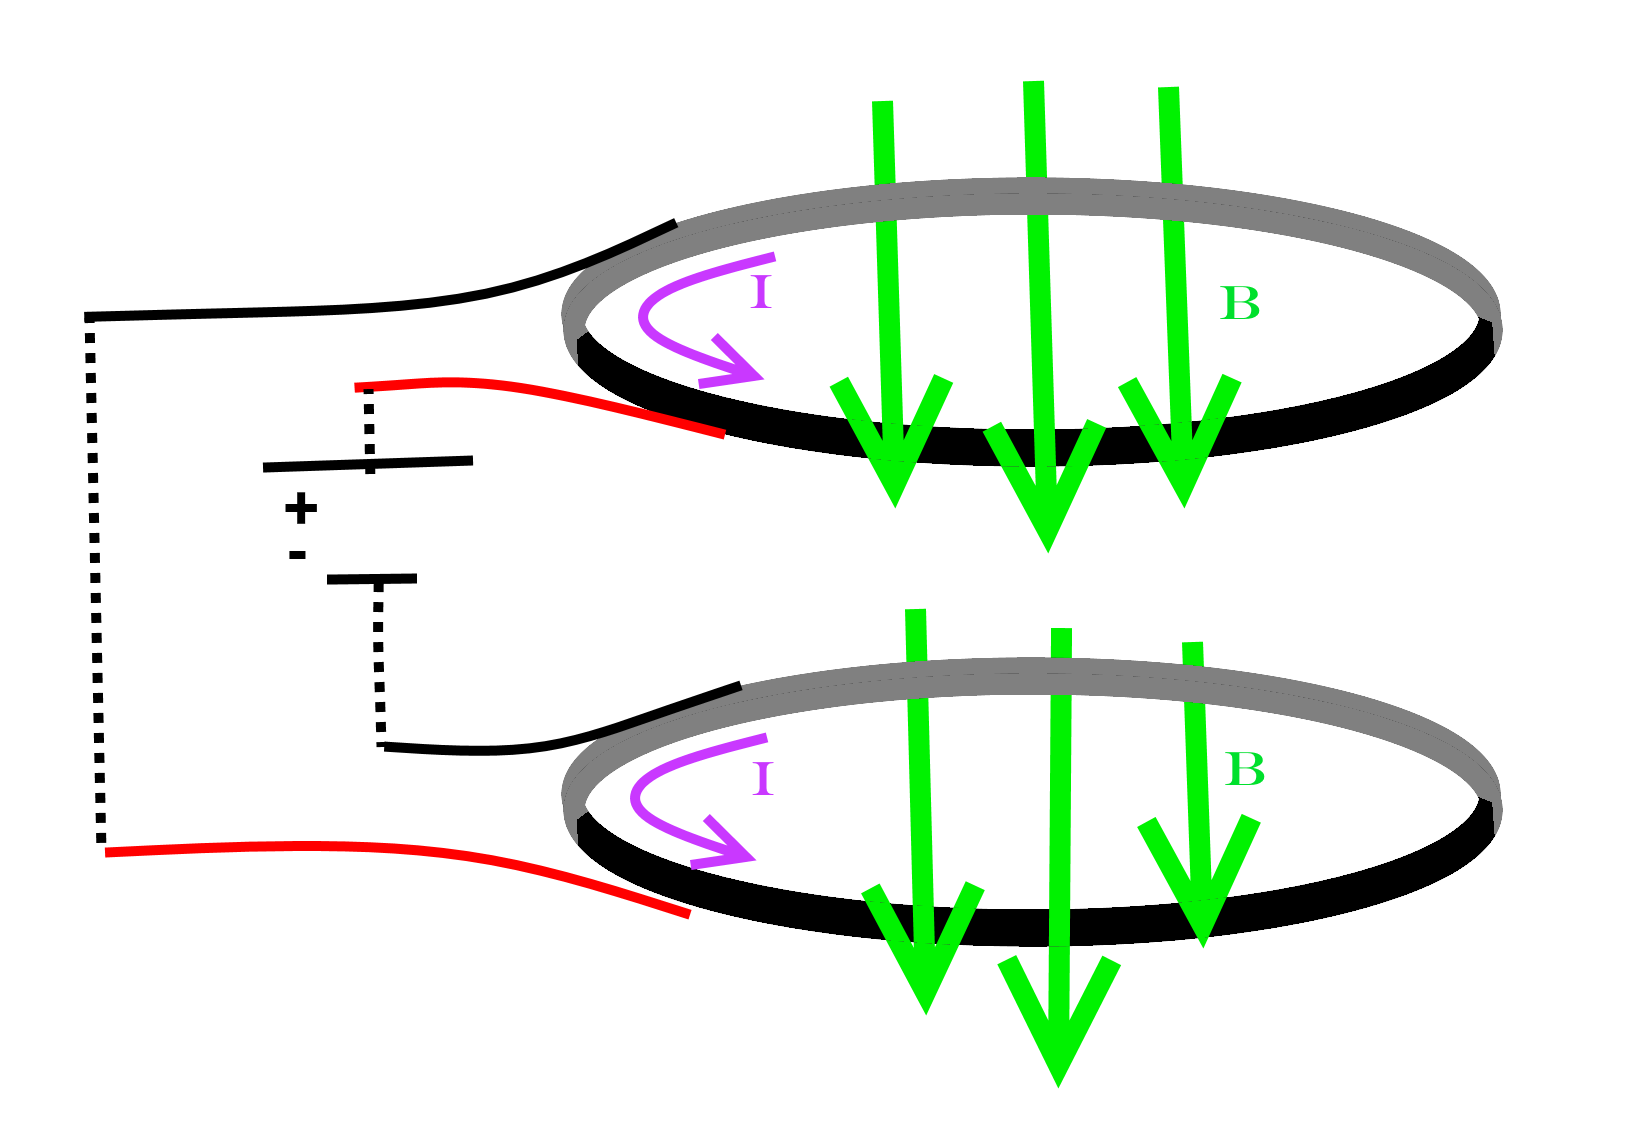
\includegraphics[width=0.5\textwidth]{circuit.png}

\captionof{figure}{Flow of current through the Helmholtz coil, oriented such
  that the produced fields are constructive.}

\label{helmholtz_circuit}
\end{figure}

\subsection{The Hall Effect Probe}

%How hall effect probe works

\qq A DC Gaussmeter (AlphaLab Model GM-1-HS) was connected to a Hall Effect Probe in
order to measure the field strength inside the Helmholtz coil. The Hall Effect
Probe contains a semiconductor junction that, when exposed to a magnetic field,
produces a voltage proportional to the field strength.


\subsection{Position Controls}

%Position Controls

\qq The position of the Hall Effect Probe can be modified in the $\rho$ direction by
sliding the ruler bar through the acrylic cube shown in figure
\ref{helmholtz_diagram}. The position can be modified in the $\phi$ direction by
rotating the ruler bar about the central pole. However, for the sake of this
experiment, this did not have to be modified because measurements were taken in
a single $\rho , z$ plane. The $z$ coordinate was modified by sliding the
acrylic cube and ruler bar up and down the central pole.


%Labeled sketch of the experimental setup
\begin{figure}[H]
\centering
% uncomment the line below to add image
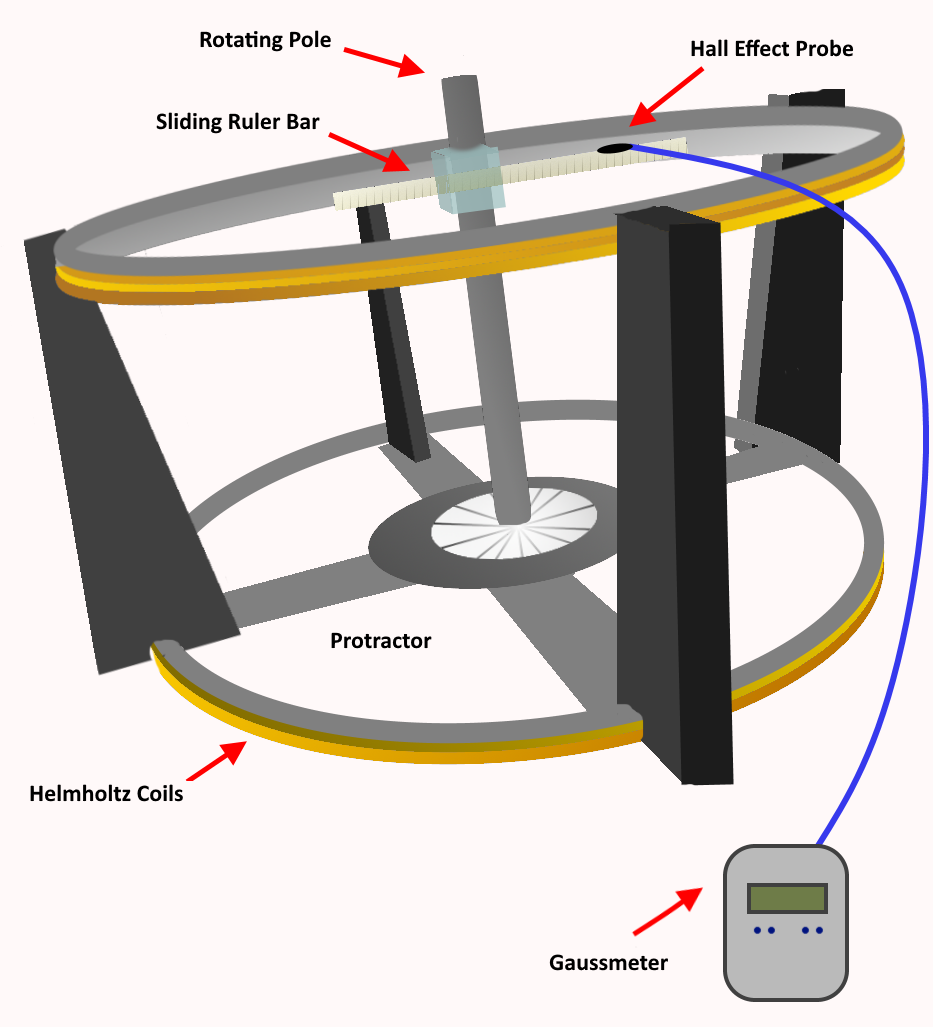
\includegraphics[width=0.5\textwidth]{helmholtz_diagram.png}
\captionof{figure}{Two concentric Helmholtz coils separated by a distance equal
  to their radius. Rotating pole and sliding ruler allow for modification of the
  probe's position.}

\label{helmholtz_diagram}
\end{figure}

\section{Procedure}


% Describe the main steps in the experimental procedures. Be sure to include any
% precautions. Sufficient details should be given such that another student can
% follow and do the experiment.
\qq Note that, per suggestion of the laboratory manual, the procedural steps of this
experiment have been omitted. The discussion section provides sufficient detail
on what actions were taken.

\subsection{Measuring the External Field}
% How the external field was measured
\qq The Helmholtz coil is oriented such that the Earth's magnetic field is parallel
to the z-axis of the coils. This allows us to produce an applied magnetic field
that is exactly anti-parallel to the Earth's field. From there, we can compute
the applied field by subtracting the Earth's field from the total resultant
field.

\qq Note that there was an apparent offset in the Gaussmeter reading, as the 0.36G
measurement for Earth's field was consistently higher than the expected value
for Earth's field of 0.24G. However, if there truly exists such an offset in the
measurement device, it would appear in both the measurement of Earth's field and
in the measurement of the total field inside the Helmholtz coil. Subtracting
these two to obtain the strength of the applied field would cancel any
contribution from such an offset.


\subsection{Procedural Modifications}

%malalligned axis
\qq Upon initial inspection of the equipment, it appeared the center pole running
along the z axis of the Helmholtz coil was misaligned. In order to mitigate this
error and ensure that coordinates were modified independently, a cord was used
to realign the pole as closely as possible to the true z axis. However, since
this alignment was not quantified, it is possible that there the pole is
misaligned to some degree. This would result in a systematic error intrinsic to
the experimental set-up. If the pole deviates from the z-axis, the
experimentally recorded z-values are underestimated, causing the experimental
field strengths to trend lower than the theoretical field strengths.

% Day-to-day current offset
\qq The majority of field strength measurements collected for the 3-dimensional
mapping were taken on the same day of experimentation. After resuming this data
collection on the next day, the values appeared to be systematically
higher. Possible causes of this offset were investigated. Before taking
measurements and intermittently during the data collection, the hall effect
probe was zeroed and observed with the power supply off in order to ensure a
consistent reading of the Earth's magnetic field. The reference measurement
taken at the start of this lab session was similar to those taken during the
previous session (zeroed field measurements were between 0.36G and 0.4G on both
days), so a discrepancy in the Earth's field strength measurement was eliminated
as the source of this error. Note that any small variation in the Earth's field
measurement could be due to misalignment of the probe (a systematic error in
measurement that would under-report the field strength) or simply a random error
in measurement due to the limited performance of the probe.

\qq An ammeter was also used to ensure a 2A current was consistently applied on both
days of data collection, thus a change in the applied current was eliminated as
a source of error. Because the source of this error was ultimately not
determined and eliminated, the effect had to be compensated for with a
procedural modification. In order to recreate the data points from the previous
lab session, the current from the power supply was modified until the field
strength matched previous measurements in several locations. This ultimately
required lowering the applied current from 2000mA to 1790mA.

\qq Upon further investigation, it appeared the current from the power supply was
unstable, as it would decrease and increase every few minutes. This produced a
source of random intrinsic error, which was mitigated by fine tuning the current
value before each measurement after the issue was discovered.


\subsection{Additional Sources of Error}

% Proximity to power supply

\qq Because the experimental set-up was restricted to a small area, the contribution
from the field produced by the power supply may be non-negligible. From the
perspective of the experimenter, the power supply sits behind and to the right
of the Helmholtz coil. Therefore, by the curling right hand rule, this would
produce an upward magnetic field on the side of the wire nearest the Helmholtz
coil. This would produce a systematic intrinsic error that causes the external
field measurements to be overestimated. Similarly, the power supply itself may
be producing a small field that could also contribute a systematic error,
although the exact effect could not be determined without knowing the
orientation of such a field.


\section{Data Analysis}
%Graphs, figures, and tables with captions
%Results with error analysis
%Calculate discrepancies from theory


\subsection{Calculating Supply Voltage}

\qq Using a multimeter, the resistance of a set of coils was measured to be
$3.4 \Omega$. In order to determine the necessary voltage to send 3A of current
through the coils, we made a simple calculation using Ohm's law.


% Calculating voltage
\begin{align*}
V &= IR \\
  &= (\SI{3}{\ampere})(\SI{3.4}{\ohm}) \\
  &= 10.2V \\
\end{align*}

% Calculating number of turns
\subsection{Determining the Number of Turns in a Coil}

\qq Further calculations will require knowing the number of turns of wire in each set of coils. When a known current $I$ is applied to a single coil, a field of strength $B_{loop}$ is produced. A value for $B_{loop}$ is calculated below, where $a$ is the radius of the loop.

\begin{align*}
B_{loop} &= \frac{\mu_0 I}{2a} \\
         &= \frac{4 \pi \times 10^{-7} Tm/A \times 2A}{2\times 0.332m} \\
         &= 3.78 \times 10^{-6} \text{ T} \\
         &= 3.78 \times 10^{-2} \text{ G} \\
\end{align*}

The applied field strength was then measured across the top set of coils, with the applied current of 2A mentioned above. The number of loops $N$ could be determined by dividing the total measured field by the field calculated for a single turn of wire.

\begin{align*}
N &= \frac{B_{measured}}{B_{loop}} \\
  &= \frac{2.75G}{3.78 \times 10^{-2}G} \\
  &= 72.66 \text{ G} \\
\end{align*}

The process was conducted on the top set of coils twice, for a parallel and anti-parallel field. These two measurements and calculations were then repeated for the bottom set of coils. Averaging these four values for $N$ and rounding to the nearest integer yields an average number of turns in a coil of $N=73$.

\subsection{The Resultant Plots}
%Theoretical calculations of axial field strength
\qq Theoretical values for what the strength of the magnetic field ought to be
within the Helmholtz coils were determined by translating Equation
\ref{eq:longBiotSavart} into Julia code, shown in lines 44-95 of the first
program in Appendix B. 

% 3D plot (theoretical)
\begin{figure}[H]
\centering
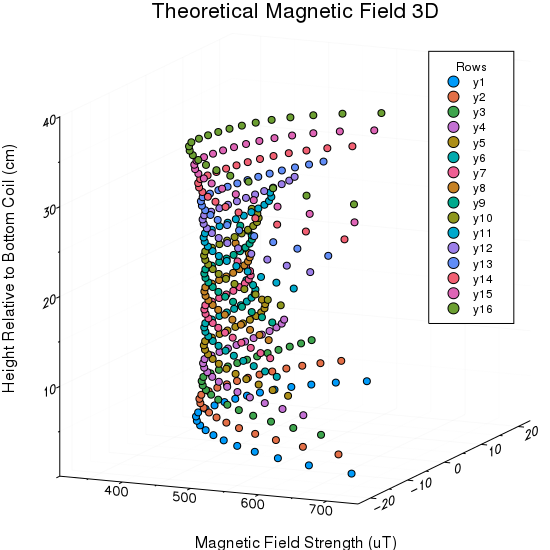
\includegraphics[width=0.5\textwidth]{3DPlotTheoretical.png}

\captionof {figure}{The theoiretical three dimensional plot calculated by using
  Symthe's deviation of the Biot-Savart Law.}

\label{Theoretical 3-D plot}
\end{figure}

% 2D plot (theoretical)

\begin{figure}[H]
  \begin{center}
    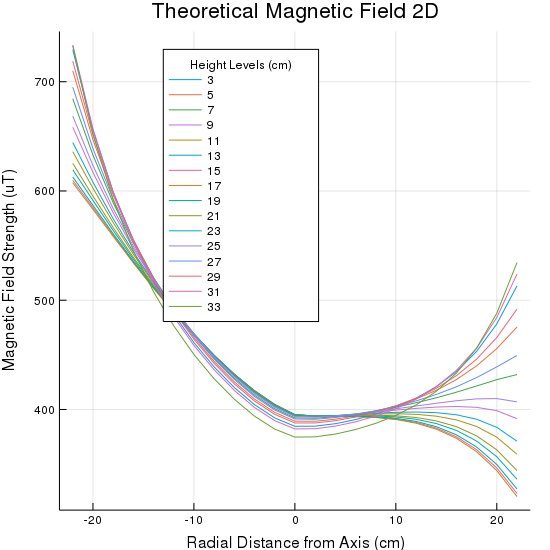
\includegraphics[width=0.5\textwidth]{2DPlotTheoretical.png}
  \end{center}
  \caption{The theoretical two dimensional used for comparison to the data
    obtained during the experimentation.}
  \label{Theoretical 2-D plot}

\end{figure}

% 3D plot (exp)
\begin{figure}[H]
\centering
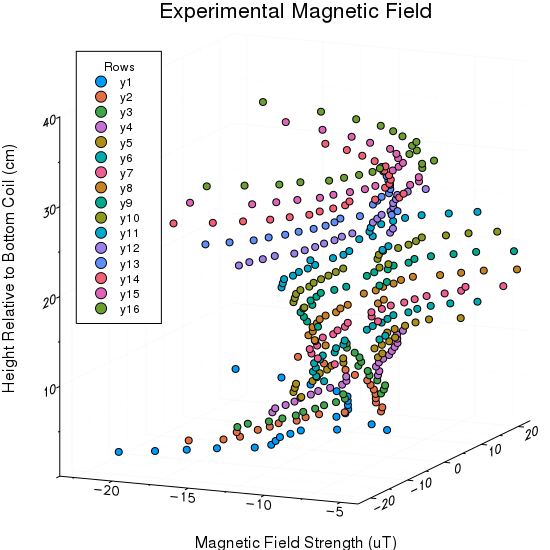
\includegraphics[width=0.5\textwidth]{3DPlotExperimental.png}

\captionof {figure}{The three dimensional plot with the data obtained during
    the experimentation. Where the magnetic field of the Helmhotz coil is mapped
    out to provide a visual of how the magnetic field is shaped and its
    strengths and differing areas. }
  \label{Experimental 3-D plot}
\end{figure}
% 2D plot (exp)
\begin{figure}[H]
\centering
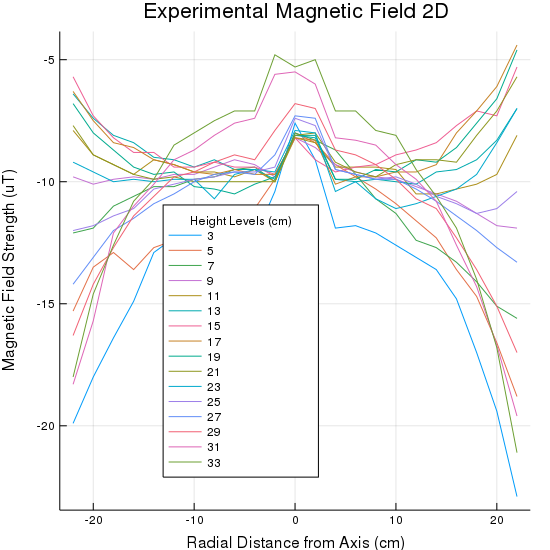
\includegraphics[width=0.5\textwidth]{2DPlotExperimental.png}
\captionof {figure}{The two dimensional plot witht the data obtained during the
  experimentation. Where each line corresponds to a differing value along the
  z-axis of the Helmholtz coil as a function of the magnetic field strength in
  $\mu$ Tesla and the radial distance from the z-axis in cm.}

\label{Experimental 2-D plot}
\end{figure}

% Calculating discrepancies

% 3D plot discrepancies 

% 2D plot discrepancies

\section{Results}
%Discuss results and uncertainties
%Compare results with theory
%Approximations to theory
\subsection{Comparing the Theoretical Plots to the Experimental Plots}
The experimental three dimensional plot does follow the theoretical
plot in the sense that the data in the mid region should be clustered
closer together than the edge regions. This is due to the uniformity
of the magnetic field in this region. Whereas the regions closest to
the coils are exposed to a greater magnetic field due to their closer
proximity to the coils themselves. The area nearest to the power
source also draws interference from the power source and the magnetic
field and thus the magnetic field is skewed to be stronger. The
experimental three dimensional plot is seemingly flipped 180 degrees
due to the fact the experiemental magnetic field was measured to be
negative while the theoretical magnetic field was calculated to be
positive.

The experimental two dimensional plot does follow the theoretical plot
in the sense that the data in the mid region is clustered close
together. The derivatives of this area of the graph approach a
plateu, this is recognized to be the center region of the coils where
the uniformity of the magnetic field is most prominent. The measured
magnetic field was determined to be much weaker than the theoretical
magnetic field. Our measured field was approximately an order of
magnitude weaker than the theoretical. The magnetic field was once
again measured to be of negative value while the theoretical magnetic
field was determined to be of positive value.

% Determine span of uniform region with 1percent margin and 5percent margin
\subsection{Determining the Span of the Uniform Region with Margins}
% Compare B field in different direction, can we say field is axial
\subsection{Comparing the directions of the Magnetic Field}


\qq When measuring at a probe height of a/2 (16cm), where 'a' is the separation
distance between the coils, the strength of the magnetic field in the 'z'
direction was measured to be -3.13 Gauss. When measuring t he magnetic field in
the 'z' direction at a probe height of 5cm, the magnetic field strength was
measure d to be -3.28 Gauss. These results follow with the theory as it is
expected that the magnetic field is p ropagated in the 'z' direction. The
measured magnetic field strength for the $\rho$ direction was -0.46 and -0.05
Gauss for a probe height of 16cm and 5cm respectfully. The measured magnetic
field strength for the $\phi$ direction was -0.51 and -0.31 Gauss for a probe
height of 16cm and 5cm respectfully. For a probe height of 16cm the percentage
for the magnitude of the magnetic field that is measured to be in th e $\rho$
direction is 14$\%$ while the percentage for the magnitude of the magnetic field
that is measur ed to be in the $\phi$ direction is 16$\%$. For a probe height of
5cm the percentage for the magnitude o f the magnetic field that is measured to
be in the $\rho$ direction is 1$\%$ while the percentage for th e magnitude of
the magnetic field that is measured to be in the $\phi$ direction is 9$\%$.The
magnetic field produced by the Helmholtz coils should be directed along the 'z'
axis. These small measuredvalues f ollow the aforementioned theoryand we can
determine that the magnetic field produced by the Helmholtz c oil is indeed
axial. Furthermore, we can determine thatthe magnetic field is axial along the
'z' direction.


\section{Conclusion}
%Brief summary, discussion of results and theory
\qq 

\section{Appendices}

\subsection{Appendix A: Data}

\begin{sidewaysfigure}
  \caption{The collected experimental data in Gauss. The top row represents the
    radial distance from the axis in centimeters, and the left column represents
    height levels in centimeters.}
  \begin{center}
    \begin{adjustwidth}{-4cm}{}
      \begin{tabular}{|r||r|r|r|r|r|r|r|r|r|r|r|r|r|r|r|r|r|r|r|r|r|r|r|}
\hline
& -22 & -20 & -18 & -16 & -14 & -12 & -10 & -8 & -6 & -4 & -2 & 0 & 2 & 4 & 6 & 8 & 10 & 12 & 14 & 16 & 18 & 20 & 22 \\
\hline
\hline
33 & -4.08 & -3.74 & -3.54 & -3.36 & -3.27 & -3.13 & -3.08 & -3.03 & -2.99 & -2.99 & -2.76 & -2.81 & -2.78 & -2.99 & -2.99 & -3.07 & -3.09 & -3.23 & -3.34 & -3.47 & -3.68 & -3.96 & -4.39 \\
31 & -4.11 & -3.85 & -3.49 & -3.38 & -3.29 & -3.19 & -3.15 & -3.09 & -3.04 & -3.02 & -2.84 & -2.83 & -2.88 & -3.1 & -3.11 & -3.13 & -3.21 & -3.27 & -3.36 & -3.54 & -3.71 & -3.95 & -4.24 \\
29 & -3.91 & -3.7 & -3.55 & -3.42 & -3.34 & -3.26 & -3.24 & -3.2 & -3.17 & -3.19 & -3.07 & -2.96 & -2.98 & -3.15 & -3.17 & -3.21 & -3.27 & -3.35 & -3.39 & -3.51 & -3.64 & -3.79 & -3.98 \\
27 & -3.7 & -3.59 & -3.48 & -3.43 & -3.37 & -3.33 & -3.28 & -3.25 & -3.24 & -3.25 & -3.17 & -3.01 & -3.02 & -3.23 & -3.25 & -3.27 & -3.27 & -3.31 & -3.36 & -3.42 & -3.48 & -3.55 & -3.61 \\
25 & -3.48 & -3.46 & -3.42 & -3.39 & -3.31 & -3.29 & -3.27 & -3.26 & -3.24 & -3.24 & -3.22 & -3.02 & -3.05 & -3.23 & -3.25 & -3.27 & -3.26 & -3.29 & -3.34 & -3.37 & -3.41 & -3.39 & -3.32 \\
23 & -3.2 & -3.24 & -3.28 & -3.27 & -3.28 & -3.27 & -3.27 & -3.35 & -3.25 & -3.23 & -3.24 & -3.07 & -3.08 & -3.32 & -3.28 & -3.35 & -3.39 & -3.37 & -3.34 & -3.31 & -3.25 & -3.12 & -2.98 \\
21 & -3.05 & -3.17 & -3.21 & -3.25 & -3.27 & -3.26 & -3.28 & -3.28 & -3.28 & -3.28 & -3.28 & -3.09 & -3.08 & -3.2 & -3.24 & -3.26 & -3.21 & -3.19 & -3.19 & -3.2 & -3.09 & -2.99 & -2.85 \\
19 & -2.96 & -3.08 & -3.15 & -3.22 & -3.25 & -3.24 & -3.3 & -3.31 & -3.33 & -3.29 & -3.26 & -3.09 & -3.09 & -3.27 & -3.27 & -3.23 & -3.24 & -3.19 & -3.2 & -3.14 & -3.04 & -2.94 & -2.74 \\
17 & -2.91 & -3.03 & -3.12 & -3.14 & -3.19 & -3.21 & -3.24 & -3.25 & -3.23 & -3.25 & -3.25 & -3.1 & -3.11 & -3.29 & -3.26 & -3.26 & -3.24 & -3.24 & -3.21 & -3.08 & -2.99 & -2.89 & -2.72 \\
15 & -2.85 & -3.01 & -3.1 & -3.16 & -3.16 & -3.22 & -3.22 & -3.2 & -3.22 & -3.22 & -3.25 & -3.1 & -3.19 & -3.24 & -3.22 & -3.21 & -3.17 & -3.15 & -3.12 & -3.05 & -2.99 & -3.01 & -2.81 \\
13 & -2.92 & -3.02 & -3.09 & -3.12 & -3.18 & -3.19 & -3.22 & -3.19 & -3.23 & -3.23 & -3.27 & -3.09 & -3.1 & -3.27 & -3.28 & -3.27 & -3.28 & -3.29 & -3.24 & -3.23 & -3.19 & -3.11 & -2.98 \\
11 & -3.07 & -3.17 & -3.21 & -3.25 & -3.19 & -3.21 & -3.24 & -3.24 & -3.26 & -3.23 & -3.28 & -3.1 & -3.12 & -3.22 & -3.22 & -3.22 & -3.23 & -3.33 & -3.33 & -3.31 & -3.29 & -3.25 & -3.09 \\
9 & -3.26 & -3.29 & -3.27 & -3.26 & -3.27 & -3.25 & -3.25 & -3.22 & -3.19 & -3.21 & -3.26 & -3.1 & -3.14 & -3.21 & -3.24 & -3.26 & -3.27 & -3.3 & -3.33 & -3.36 & -3.41 & -3.46 & -3.47 \\
7 & -3.49 & -3.47 & -3.38 & -3.34 & -3.3 & -3.3 & -3.27 & -3.26 & -3.23 & -3.22 & -3.28 & -3.08 & -3.11 & -3.15 & -3.25 & -3.35 & -3.41 & -3.52 & -3.55 & -3.61 & -3.69 & -3.79 & -3.84 \\
5 & -3.81 & -3.63 & -3.57 & -3.64 & -3.55 & -3.52 & -3.51 & -3.44 & -3.43 & -3.39 & -3.27 & -3.08 & -3.12 & -3.21 & -3.26 & -3.31 & -3.37 & -3.44 & -3.51 & -3.64 & -3.75 & -3.94 & -4.16 \\
3 & -4.27 & -4.08 & -3.92 & -3.77 & -3.57 & -3.51 & -3.53 & -3.55 & -3.53 & -3.51 & -3.32 & -3.04 & -3.19 & -3.47 & -3.46 & -3.49 & -3.54 & -3.59 & -3.64 & -3.76 & -3.98 & -4.22 & -4.57 \\
    \hline
      \end{tabular}
    \end{adjustwidth}
  \end{center}
\end{sidewaysfigure}

% page number overlaps with table
\thispagestyle{empty}

\subsection{Appendix B: Source Code}

%\label{lst:BiotSavartTheoretical}
\inputminted{julia}{BiotSavartTheoretical.jl}

%\label{lst:BiotSavartExperimental}
\inputminted{julia}{BiotSavartExperimental.jl}

%\label{lst:TheoreticalVsExperimental}
\inputminted{julia}{TheoreticalVsExperimental.jl}


\end{document}
